% ============================================================
% Reporte: Conversión de Imagen BMP a Escala de Grises
%          en Ensamblador x64 (MASM) con Interfaz C++
% Autor: Edson Joel Carrera Avila
% ============================================================

\documentclass[12pt, letterpaper]{article}

\usepackage[utf8]{inputenc}
\usepackage[T1]{fontenc}
\usepackage[spanish]{babel}
\usepackage{geometry}
\usepackage{graphicx}
\usepackage{listings}
\usepackage{xcolor}
\usepackage{booktabs}
\usepackage{amsmath}
\usepackage{hyperref}
\usepackage{xurl}
\usepackage{fancyhdr}
\usepackage{float}
\usepackage{caption}
\usepackage{tikz}
\usetikzlibrary{shapes.geometric, arrows.meta, positioning}

\geometry{top=2.5cm, bottom=2.5cm, left=3cm, right=2.5cm}

% --- Colores y estilo de código ---
\definecolor{codegray}{rgb}{0.95,0.95,0.95}
\definecolor{codegreen}{rgb}{0.0,0.5,0.0}
\definecolor{codeblue}{rgb}{0.0,0.0,0.65}
\definecolor{codepurple}{rgb}{0.45,0.0,0.55}

\lstdefinelanguage{MASM}{
    morekeywords={PROC,ENDP,END,PUBLIC,PUSH,POP,MOV,ADD,SUB,CALL,RET,JMP,
                  JE,JB,JA,JGE,JLE,JNZ,JZ,DEC,INC,CMP,TEST,XOR,EXTERN,
                  BYTE,DWORD,QWORD,XMMWORD,YMMWORD,PTR,
                  RAX,RBX,RCX,RDX,RSI,RDI,RSP,RBP,R8,R9,R10,R11,R8D,R9D,R10D,R11D,R11B,
                  XMM0,XMM1,YMM0,YMM1,ST,
                  MOVZX,IMUL,SHR,SHL,
                  .code,.data},
    sensitive=false,
    morecomment=[l]{;}
}

\lstdefinelanguage{CPP}{
    morekeywords={int,float,size_t,const,static,alignas,printf,using,namespace,
                  extern,include,return,for,unsigned,uint8_t,uint16_t,uint32_t,
                  uint64_t,int32_t,struct,reinterpret_cast,vector,string,cout,
                  endl,ifstream,ofstream,ios,binary,cerr,abs,pragma,pack,push,pop,data,seekg,seekp,
                  beg,read,write,close,size,sizeof,char,if,else,bool,true,false},
    sensitive=true,
    morecomment=[l]{//},
    morestring=[b]"
}

\lstset{
    backgroundcolor=\color{codegray},
    basicstyle=\ttfamily\footnotesize,
    keywordstyle=\color{codeblue}\bfseries,
    commentstyle=\color{codegreen}\itshape,
    numbers=left, numberstyle=\tiny\color{gray}, numbersep=8pt,
    frame=single, rulecolor=\color{gray!50},
    breaklines=true, captionpos=b, tabsize=4,
    showstringspaces=false,
    literate=
        {á}{{\'a}}1 {é}{{\'e}}1 {í}{{\'i}}1 {ó}{{\'o}}1 {ú}{{\'u}}1
        {Á}{{\'A}}1 {É}{{\'E}}1 {Í}{{\'I}}1 {Ó}{{\'O}}1 {Ú}{{\'U}}1
        {ñ}{{\~n}}1 {Ñ}{{\~N}}1
}

% --- Encabezado ---
\pagestyle{fancy}
\fancyhf{}
\rhead{Proyecto 01 — Grayscale}
\lhead{\textit{Edson Joel Carrera Avila}}
\cfoot{\thepage}
\renewcommand{\headrulewidth}{0.5pt}

% ============================================================
\begin{document}

% --- Portada ---
\begin{titlepage}
    \centering
    \vspace*{1.5cm}

    {\Large \textbf{Universidad Autónoma de la Ciudad de México}}\\[0.3cm]
    {\large Licenciatura en Ingeniería de Software}\\[0.2cm]
    {\large Arquitectura de Computadoras}\\[2.5cm]

    \rule{\linewidth}{0.5pt}\\[0.4cm]
    {\LARGE \bfseries Proyecto 01}\\[0.3cm]
    {\Large Conversión de Imagen BMP a Escala de Grises en Ensamblador x64}\\[0.3cm]
    \rule{\linewidth}{0.5pt}\\[2cm]

    \begin{flushleft}
        \textbf{Alumno:} Edson Joel Carrera Avila \\[0.3cm]
        \textbf{Grupo:} 302 \\[0.3cm]
        \textbf{Profesor:} Prof. Mtro. Omar Nieto Crisóstomo \\[0.3cm]
        \textbf{Fecha:} \today
    \end{flushleft}
    \vfill
\end{titlepage}

\tableofcontents
\newpage

% ============================================================
\section{Introducción}

Este proyecto consiste en \textbf{leer una imagen en formato BMP de 24 bits}, convertir cada uno de sus píxeles a un tono de gris equivalente usando una rutina escrita en \textbf{ensamblador x64 (MASM)}, y escribir el resultado en un nuevo archivo BMP. El programa principal en C++ se encarga de abrir el archivo, validar la cabecera, recorrer las filas de píxeles, invocar la rutina ensambladora con cada fila y finalmente guardar el archivo de salida.

\subsection*{¿Qué es el formato BMP?}

\textbf{BMP} (\textit{BitMap}), también llamado \textbf{DIB} (\textit{Device-Independent Bitmap}), es un formato de archivo desarrollado por Microsoft para almacenar mapas de bits sin compresión. Su estructura básica consta de cuatro bloques contiguos:

\begin{enumerate}
    \item \textbf{Bitmap File Header} (\texttt{BMPHeader}, 14 bytes): identifica el archivo con la firma ASCII \texttt{"BM"} (\texttt{0x4D42}) y declara el tamaño total y el desplazamiento (\texttt{offset\_data}) hasta donde comienzan los píxeles \cite{fileformat_bmp}.
    \item \textbf{Bitmap Info Header} (\texttt{DIBHeader}, normalmente 40 bytes para \texttt{BITMAPINFOHEADER}): describe las dimensiones (\texttt{width}, \texttt{height}), el número de bits por píxel (\texttt{bit\_count}), el tipo de compresión y otras propiedades \cite{microsoft_bitmapinfoheader}.
    \item \textbf{Color Palette} (opcional): tabla de colores presente cuando \texttt{bit\_count} es menor a 24. En imágenes de 24 bits \textbf{no existe paleta}, los píxeles guardan sus colores explícitamente.
    \item \textbf{Pixel Array}: los datos de la imagen propiamente dichos.
\end{enumerate}

\subsection*{¿Cómo se almacenan los píxeles en un BMP de 24 bits?}

En un BMP de 24 bits cada píxel ocupa 3 bytes y se almacena en el orden \textbf{BGR} (no RGB): primero el byte del canal Azul, luego el Verde y finalmente el Rojo \cite{fileformat_bmp}. Este orden invertido proviene de la representación natural de un entero de 32 bits en arquitecturas \textit{little-endian} (Intel/AMD), donde los bytes menos significativos quedan en las direcciones más bajas.

Además, el estándar BMP exige que cada fila (\textit{scan line}) tenga un tamaño en bytes \textbf{múltiplo de 4} \cite{microsoft_bitmapinfo}. Si el ancho en píxeles multiplicado por 3 no es divisible entre 4, se añaden bytes de \textbf{relleno} (\textit{padding}) al final de la fila. El cálculo del relleno es:

\begin{equation}
    \text{padding} = (4 - (\text{width} \times 3 \bmod 4)) \bmod 4
\end{equation}

\begin{equation}
    \text{row\_stride} = \text{width} \times 3 + \text{padding}
\end{equation}

Por ejemplo, una imagen de 100 píxeles de ancho tiene filas de $100 \times 3 = 300$ bytes, que ya es múltiplo de 4, por lo que no necesita relleno. Pero una imagen de 33 píxeles de ancho tendría filas de $33 \times 3 = 99$ bytes, y necesita un byte de relleno para alcanzar los 100 bytes \cite{fileformat_bmp}.

Otra peculiaridad: las filas se almacenan \textbf{de abajo hacia arriba} cuando la altura (\texttt{biHeight}) es positiva. Es decir, la primera fila del archivo corresponde a la fila más baja de la imagen. Si \texttt{biHeight} es negativa, las filas se almacenan de arriba hacia abajo (\textit{top-down DIB}) \cite{microsoft_bitmapinfoheader}.

\subsection*{¿Por qué los pesos $0.299$, $0.587$, $0.114$?}

Los pesos $0.299$, $0.587$ y $0.114$ provienen del estándar \textbf{ITU-R BT.601} de la Unión Internacional de Telecomunicaciones.

\begin{equation}
    Y' = 0.299\,R' + 0.587\,G' + 0.114\,B'
\end{equation}

Estos coeficientes reflejan la \textbf{sensibilidad relativa del ojo humano} a cada color: el verde aporta cerca del 59\,\% de la luminosidad percibida, el rojo el 30\,\%, y el azul apenas el 11\,\%. Por eso, un simple promedio aritmético $\frac{R+G+B}{3}$ produce imágenes que se ven incorrectas (cielos demasiado claros, vegetación demasiado oscura).

\subsection*{¿Por qué multiplicar por 256 los pesos?}

El procesador trabaja muy eficientemente con \textbf{aritmética entera}, mientras que las multiplicaciones en punto flotante son notoriamente más lentas. Una optimización clásica consiste en \textbf{escalar los pesos por una potencia de 2} para evitar el uso de la FPU:

\begin{equation}
    Y \approx \frac{29\,B + 150\,G + 77\,R}{256}
\end{equation}

donde $29 \approx 0.114 \times 256$, $150 \approx 0.587 \times 256$ y $77 \approx 0.299 \times 256$. La suma de los pesos enteros es exactamente $29 + 150 + 77 = 256 = 2^8$, lo que permite reemplazar la división final por un \textbf{desplazamiento a la derecha} de 8 bits (\texttt{SHR r11d, 8}), una de las instrucciones más rápidas del procesador \cite{intel_manual}. Esta es exactamente la estrategia usada en \texttt{grayscale.asm}.

% ============================================================
\section{Organización del proyecto}

El proyecto se compila como una aplicación de consola \textbf{x64} en Visual Studio con el conjunto de herramientas \texttt{v143}. La plataforma debe ser obligatoriamente \textbf{x64} porque las rutinas usan la convención de llamadas Microsoft x64 (\texttt{RCX}, \texttt{RDX}, \texttt{R8}) \cite{msft_x64_calling}.

\begin{figure}[H]
    \centering
    \resizebox{0.55\textwidth}{!}{%
        \begin{tikzpicture}[
            node distance=1.0cm and 2.0cm,
            startstop/.style={rectangle, rounded corners, draw=black, fill=blue!15,
                              minimum width=3.8cm, minimum height=0.8cm, align=center},
            process/.style  ={rectangle, draw=black, fill=yellow!20,
                              minimum width=4.2cm, minimum height=0.8cm, align=center},
            asmstep/.style  ={rectangle, draw=black, fill=red!15,
                              minimum width=4.2cm, minimum height=0.8cm, align=center},
            decision/.style ={diamond, draw=black, fill=orange!25,
                              minimum width=2.8cm, minimum height=0.8cm, align=center,
                              aspect=2},
            arrow/.style    ={-{Stealth[length=5pt]}, thick}
        ]
        \node[startstop] (inicio)  {Inicio (main)};
        \node[process, below=of inicio]  (abrir)   {Abrir \texttt{input.bmp}};
        \node[process, below=of abrir]   (val)     {Leer y validar cabeceras\\(firma BM, bit\_count == 24)};
        \node[process, below=of val]     (pad)     {Calcular padding\\y row\_stride};
        \node[process, below=of pad]     (read)    {Cargar todos los píxeles\\en \texttt{input\_data}};
        \node[process, below=of read]    (loop)    {Para cada fila $y$};
        \node[asmstep, below=of loop]    (asm)     {Llamar a \texttt{conversion\_grayscale}\\(rcx=row\_in, rdx=row\_out, r8=width)};
        \node[process, below=of asm]     (copypad) {Copiar bytes de padding\\sin modificar};
        \node[decision, below=of copypad](more)    {¿Más filas?};
        \node[process, below=of more]    (write)   {Escribir cabeceras y píxeles\\en \texttt{output.bmp}};
        \node[startstop, below=of write] (fin)     {Fin};

        \draw[arrow] (inicio)  -- (abrir);
        \draw[arrow] (abrir)   -- (val);
        \draw[arrow] (val)     -- (pad);
        \draw[arrow] (pad)     -- (read);
        \draw[arrow] (read)    -- (loop);
        \draw[arrow] (loop)    -- (asm);
        \draw[arrow] (asm)     -- (copypad);
        \draw[arrow] (copypad) -- (more);
        \draw[arrow] (more.east) -- ++(2.5,0) |- node[right, pos=0.25]{\small Sí} (loop.east);
        \draw[arrow] (more)    -- node[right]{\small No} (write);
        \draw[arrow] (write)   -- (fin);
        \end{tikzpicture}
    }
    \caption{Diagrama de flujo del procesamiento BMP fila por fila}
\end{figure}

% ============================================================
\section{Anatomía del archivo BMP}

\subsection{Bitmap File Header (14 bytes)}

\begin{table}[H]
    \centering
    \begin{tabular}{@{}lllp{6cm}@{}}
        \toprule
        \textbf{Offset} & \textbf{Tamaño} & \textbf{Campo} & \textbf{Descripción} \\
        \midrule
        \texttt{0x00} & 2 & \texttt{file\_type}   & Firma \texttt{"BM"} ($\texttt{0x4D42}$) \\
        \texttt{0x02} & 4 & \texttt{file\_size}   & Tamaño total del archivo en bytes \\
        \texttt{0x06} & 2 & \texttt{reserved1}    & Reservado, siempre 0 \\
        \texttt{0x08} & 2 & \texttt{reserved2}    & Reservado, siempre 0 \\
        \texttt{0x0A} & 4 & \texttt{offset\_data} & Desplazamiento al inicio del array de píxeles \\
        \bottomrule
    \end{tabular}
    \caption{Estructura del \texttt{BMPHeader} según la especificación de Microsoft \cite{microsoft_bmp}}
\end{table}

\subsection{DIB Header / BITMAPINFOHEADER (40 bytes)}

\begin{table}[H]
    \centering
    \begin{tabular}{@{}lllp{5.5cm}@{}}
        \toprule
        \textbf{Offset} & \textbf{Tamaño} & \textbf{Campo} & \textbf{Descripción} \\
        \midrule
        \texttt{0x0E} & 4 & \texttt{size}                & Tamaño de la cabecera (típicamente 40) \\
        \texttt{0x12} & 4 & \texttt{width}               & Ancho en píxeles \\
        \texttt{0x16} & 4 & \texttt{height}              & Alto en píxeles (positivo = bottom-up) \\
        \texttt{0x1A} & 2 & \texttt{planes}              & Siempre 1 \\
        \texttt{0x1C} & 2 & \texttt{bit\_count}          & Bits por píxel (24 en este proyecto) \\
        \texttt{0x1E} & 4 & \texttt{compression}         & 0 = sin compresión (BI\_RGB) \\
        \texttt{0x22} & 4 & \texttt{size\_image}         & Tamaño del array de píxeles \\
        \texttt{0x26} & 4 & \texttt{x\_pixels\_per\_meter} & Resolución horizontal \\
        \texttt{0x2A} & 4 & \texttt{y\_pixels\_per\_meter} & Resolución vertical \\
        \texttt{0x2E} & 4 & \texttt{colors\_used}        & Colores usados (0 = todos) \\
        \texttt{0x32} & 4 & \texttt{colors\_important}   & Colores importantes \\
        \bottomrule
    \end{tabular}
    \caption{Estructura del \texttt{DIBHeader} (BITMAPINFOHEADER) \cite{microsoft_bitmapinfoheader}}
\end{table}

\subsection*{El uso de \texttt{\#pragma pack(push, 1)}}

El programa principal usa la directiva \texttt{\#pragma pack(push, 1)} para garantizar que el compilador \textbf{no inserte bytes de relleno} entre los campos de las estructuras. Sin esta directiva, el compilador podría alinear los campos a fronteras naturales de 4 u 8 bytes para optimizar accesos a memoria \cite{wikipedia_data_alignment}, lo que rompería completamente el mapeo binario con el archivo BMP en disco: por ejemplo, el campo \texttt{file\_size} debe estar exactamente en el offset \texttt{0x02}, no en \texttt{0x04} como ocurriría con alineación natural.

% ============================================================
\section{Código fuente}

\subsection{Programa principal (main.cpp)}

El programa principal se encarga de toda la lógica de archivos (apertura, validación, padding, escritura) y delega a ensamblador únicamente la transformación píxel a píxel.

\begin{lstlisting}[language=CPP, caption={Definición de las cabeceras BMP empaquetadas a 1 byte}]
#pragma pack(push, 1)
struct BMPHeader {
    uint16_t file_type{0x4D42}; // Firma 'BM'
    uint32_t file_size{0};
    uint16_t reserved1{0};
    uint16_t reserved2{0};
    uint32_t offset_data{0};
};

struct DIBHeader {
    uint32_t size{0};
    int32_t  width{0};
    int32_t  height{0};
    uint16_t planes{1};
    uint16_t bit_count{0};
    uint32_t compression{0};
    uint32_t size_image{0};
    int32_t  x_pixels_per_meter{0};
    int32_t  y_pixels_per_meter{0};
    uint32_t colors_used{0};
    uint32_t colors_important{0};
};
#pragma pack(pop)
\end{lstlisting}

\begin{lstlisting}[language=CPP, caption={Cálculo del padding y procesamiento fila por fila}]
int width  = dib_header.width;
int height = abs(dib_header.height);

int row_width_bytes = width * 3;
int padding         = (4 - (row_width_bytes % 4)) % 4;
int row_stride      = row_width_bytes + padding;

vector<uint8_t> input_data(row_stride * height);
file.read(reinterpret_cast<char*>(input_data.data()), input_data.size());

vector<uint8_t> output_data(input_data.size());

for (int y = 0; y < height; ++y) {
    uint8_t* row_in  = input_data.data()  + (y * row_stride);
    uint8_t* row_out = output_data.data() + (y * row_stride);

    conversion_grayscale(row_in, row_out, width);

    // Conservar los bytes de padding originales
    for (int p = 0; p < padding; ++p) {
        row_out[row_width_bytes + p] = row_in[row_width_bytes + p];
    }
}
\end{lstlisting}

\subsection{Módulo ensamblador (grayscale.asm)}

El módulo ensamblador implementa la conversión píxel a píxel siguiendo la fórmula entera $\frac{29\,B + 150\,G + 77\,R}{256}$.

\begin{lstlisting}[language=MASM, caption={Rutina \texttt{conversion\_grayscale} completa}]
conversion_grayscale PROC
    test r8, r8                    ; hay píxeles que procesar?
    jz   fin                       ; si no, salir

bucle:
    ; --- PASO 1: cargar los 3 canales (BGR) del píxel actual ---
    movzx r9d,  byte ptr [rcx]     ; B (azul,  offset 0)
    movzx r10d, byte ptr [rcx+1]   ; G (verde, offset 1)
    movzx r11d, byte ptr [rcx+2]   ; R (rojo,  offset 2)

    ; --- PASO 2: multiplicar cada canal por su peso ---
    imul r9d,  29                  ; B * 29
    imul r10d, 150                 ; G * 150
    imul r11d, 77                  ; R * 77

    ; --- PASO 3: sumar los tres productos ---
    add r11d, r10d                 ; R*77 + G*150
    add r11d, r9d                  ; + B*29

    ; --- PASO 4: dividir por 256 (shift derecho de 8 bits) ---
    shr r11d, 8                    ; gris = (29B + 150G + 77R) >> 8

    ; --- PASO 5: escribir el mismo gris en los 3 canales de salida ---
    mov byte ptr [rdx],   r11b
    mov byte ptr [rdx+1], r11b
    mov byte ptr [rdx+2], r11b

    ; --- PASO 6: avanzar al siguiente píxel (3 bytes) ---
    add rcx, 3
    add rdx, 3

    ; --- PASO 7: decrementar contador y repetir ---
    dec r8
    jnz bucle

fin:
    ret
conversion_grayscale ENDP
\end{lstlisting}

% ============================================================
\section{Instrucciones x86/x64 utilizadas}

\subsection{Propósito y aritmética}

\begin{table}[H]
    \centering
    \begin{tabular}{@{}lp{10cm}@{}}
        \toprule
        \textbf{Instrucción} & \textbf{Operación} \\
        \midrule
        \texttt{TEST}  & Realiza una AND lógica entre dos operandos sin almacenar el resultado; sólo afecta banderas. Se usa para detectar si \texttt{R8} es cero al inicio \cite{intel_manual}. \\
        \texttt{MOVZX} & \textit{Move with Zero-eXtend}: copia un byte/word a un registro más grande rellenando los bits superiores con ceros. Imprescindible antes de \texttt{IMUL} para evitar interpretar los bits altos como basura. \\
        \texttt{IMUL}  & \textit{Integer Multiply}: multiplicación entera con signo. Aquí se usa con un inmediato como segundo operando (forma de 3 operandos). \\
        \texttt{ADD}   & Suma entera (acumula los productos parciales). \\
        \texttt{SHR}   & \textit{Shift Right}: desplaza los bits a la derecha. Una división por $2^n$ se reduce a un \texttt{SHR n}, mucho más rápido que una división entera. \\
        \texttt{MOV}   & Mueve un byte de un registro a memoria (escritura del píxel de salida). \\
        \bottomrule
    \end{tabular}
    \caption{Instrucciones aritméticas y de movimiento}
\end{table}

\subsection{Control de flujo}

\begin{table}[H]
    \centering
    \begin{tabular}{@{}lp{10cm}@{}}
        \toprule
        \textbf{Instrucción} & \textbf{Operación} \\
        \midrule
        \texttt{JZ}    & \textit{Jump if Zero}: salta si la bandera ZF está activada (resultado anterior fue cero). \\
        \texttt{DEC}   & Decrementa un registro en 1 y actualiza ZF si el resultado es cero. \\
        \texttt{JNZ}   & \textit{Jump if Not Zero}: salta si ZF no está activada. Aquí mantiene vivo el bucle. \\
        \texttt{RET}   & Retorna al llamador (\texttt{main.cpp}). \\
        \bottomrule
    \end{tabular}
    \caption{Instrucciones de control de flujo del bucle}
\end{table}

% ============================================================
\section{El rol de los registros}

\subsection{Convención de llamadas Microsoft x64}

A diferencia de la \textit{cdecl} de 32 bits (parámetros en la pila), en x64 los primeros cuatro argumentos enteros viajan en registros específicos \cite{msft_x64_calling}:

\begin{table}[H]
    \centering
    \begin{tabular}{@{}lll@{}}
        \toprule
        \textbf{Registro} & \textbf{Parámetro} & \textbf{Descripción} \\
        \midrule
        \texttt{RCX} & \texttt{uint8\_t* input}        & Puntero a la fila de entrada (BGR) \\
        \texttt{RDX} & \texttt{uint8\_t* output}       & Puntero a la fila de salida (gris) \\
        \texttt{R8}  & \texttt{uint64\_t pixel\_count} & Número de píxeles a procesar (= ancho) \\
        \bottomrule
    \end{tabular}
    \caption{Mapa de parámetros para la convención Microsoft x64}
\end{table}

\subsection{Registros internos}

\begin{table}[H]
    \centering
    \begin{tabular}{@{}llp{6.5cm}@{}}
        \toprule
        \textbf{Registro} & \textbf{Subregistro 32-bit} & \textbf{Rol} \\
        \midrule
        \texttt{R9}  & \texttt{R9D}  & Almacena el canal $B$ extendido a 32 bits. Tras \texttt{IMUL 29}, contiene $29B$. \\
        \texttt{R10} & \texttt{R10D} & Almacena el canal $G$. Tras \texttt{IMUL 150}, contiene $150G$. \\
        \texttt{R11} & \texttt{R11D} / \texttt{R11B} & Acumulador final del cálculo. \texttt{R11D} guarda la suma ponderada y, tras \texttt{SHR 8}, su byte bajo \texttt{R11B} contiene el valor de gris [0--255]. \\
        \bottomrule
    \end{tabular}
    \caption{Uso de los registros generales dentro de la rutina}
\end{table}

\subsection*{¿Por qué \texttt{R11B} es exactamente el valor de gris?}

Después de \texttt{IMUL} cada producto cabe en menos de 16 bits ($255 \times 150 = 38250 \approx 2^{16}$). La suma de los tres productos cabe holgadamente en 32 bits ($255 \times 256 = 65280$). Al dividir entre 256 con \texttt{SHR 8}, el resultado está garantizado en el rango $[0, 255]$, por lo que su \textbf{byte bajo} \texttt{R11B} es directamente el valor de gris a escribir.

% ============================================================
\section{Ejemplo de ejecución}

\subsection{Imagen de entrada}

Como caso de prueba se utiliza una fotografía en color, guardada como BMP de 24 bits con cualquier editor (Paint, GIMP, Photoshop) en la ruta \texttt{src/input.bmp}.

\begin{figure}[H]
    \centering
    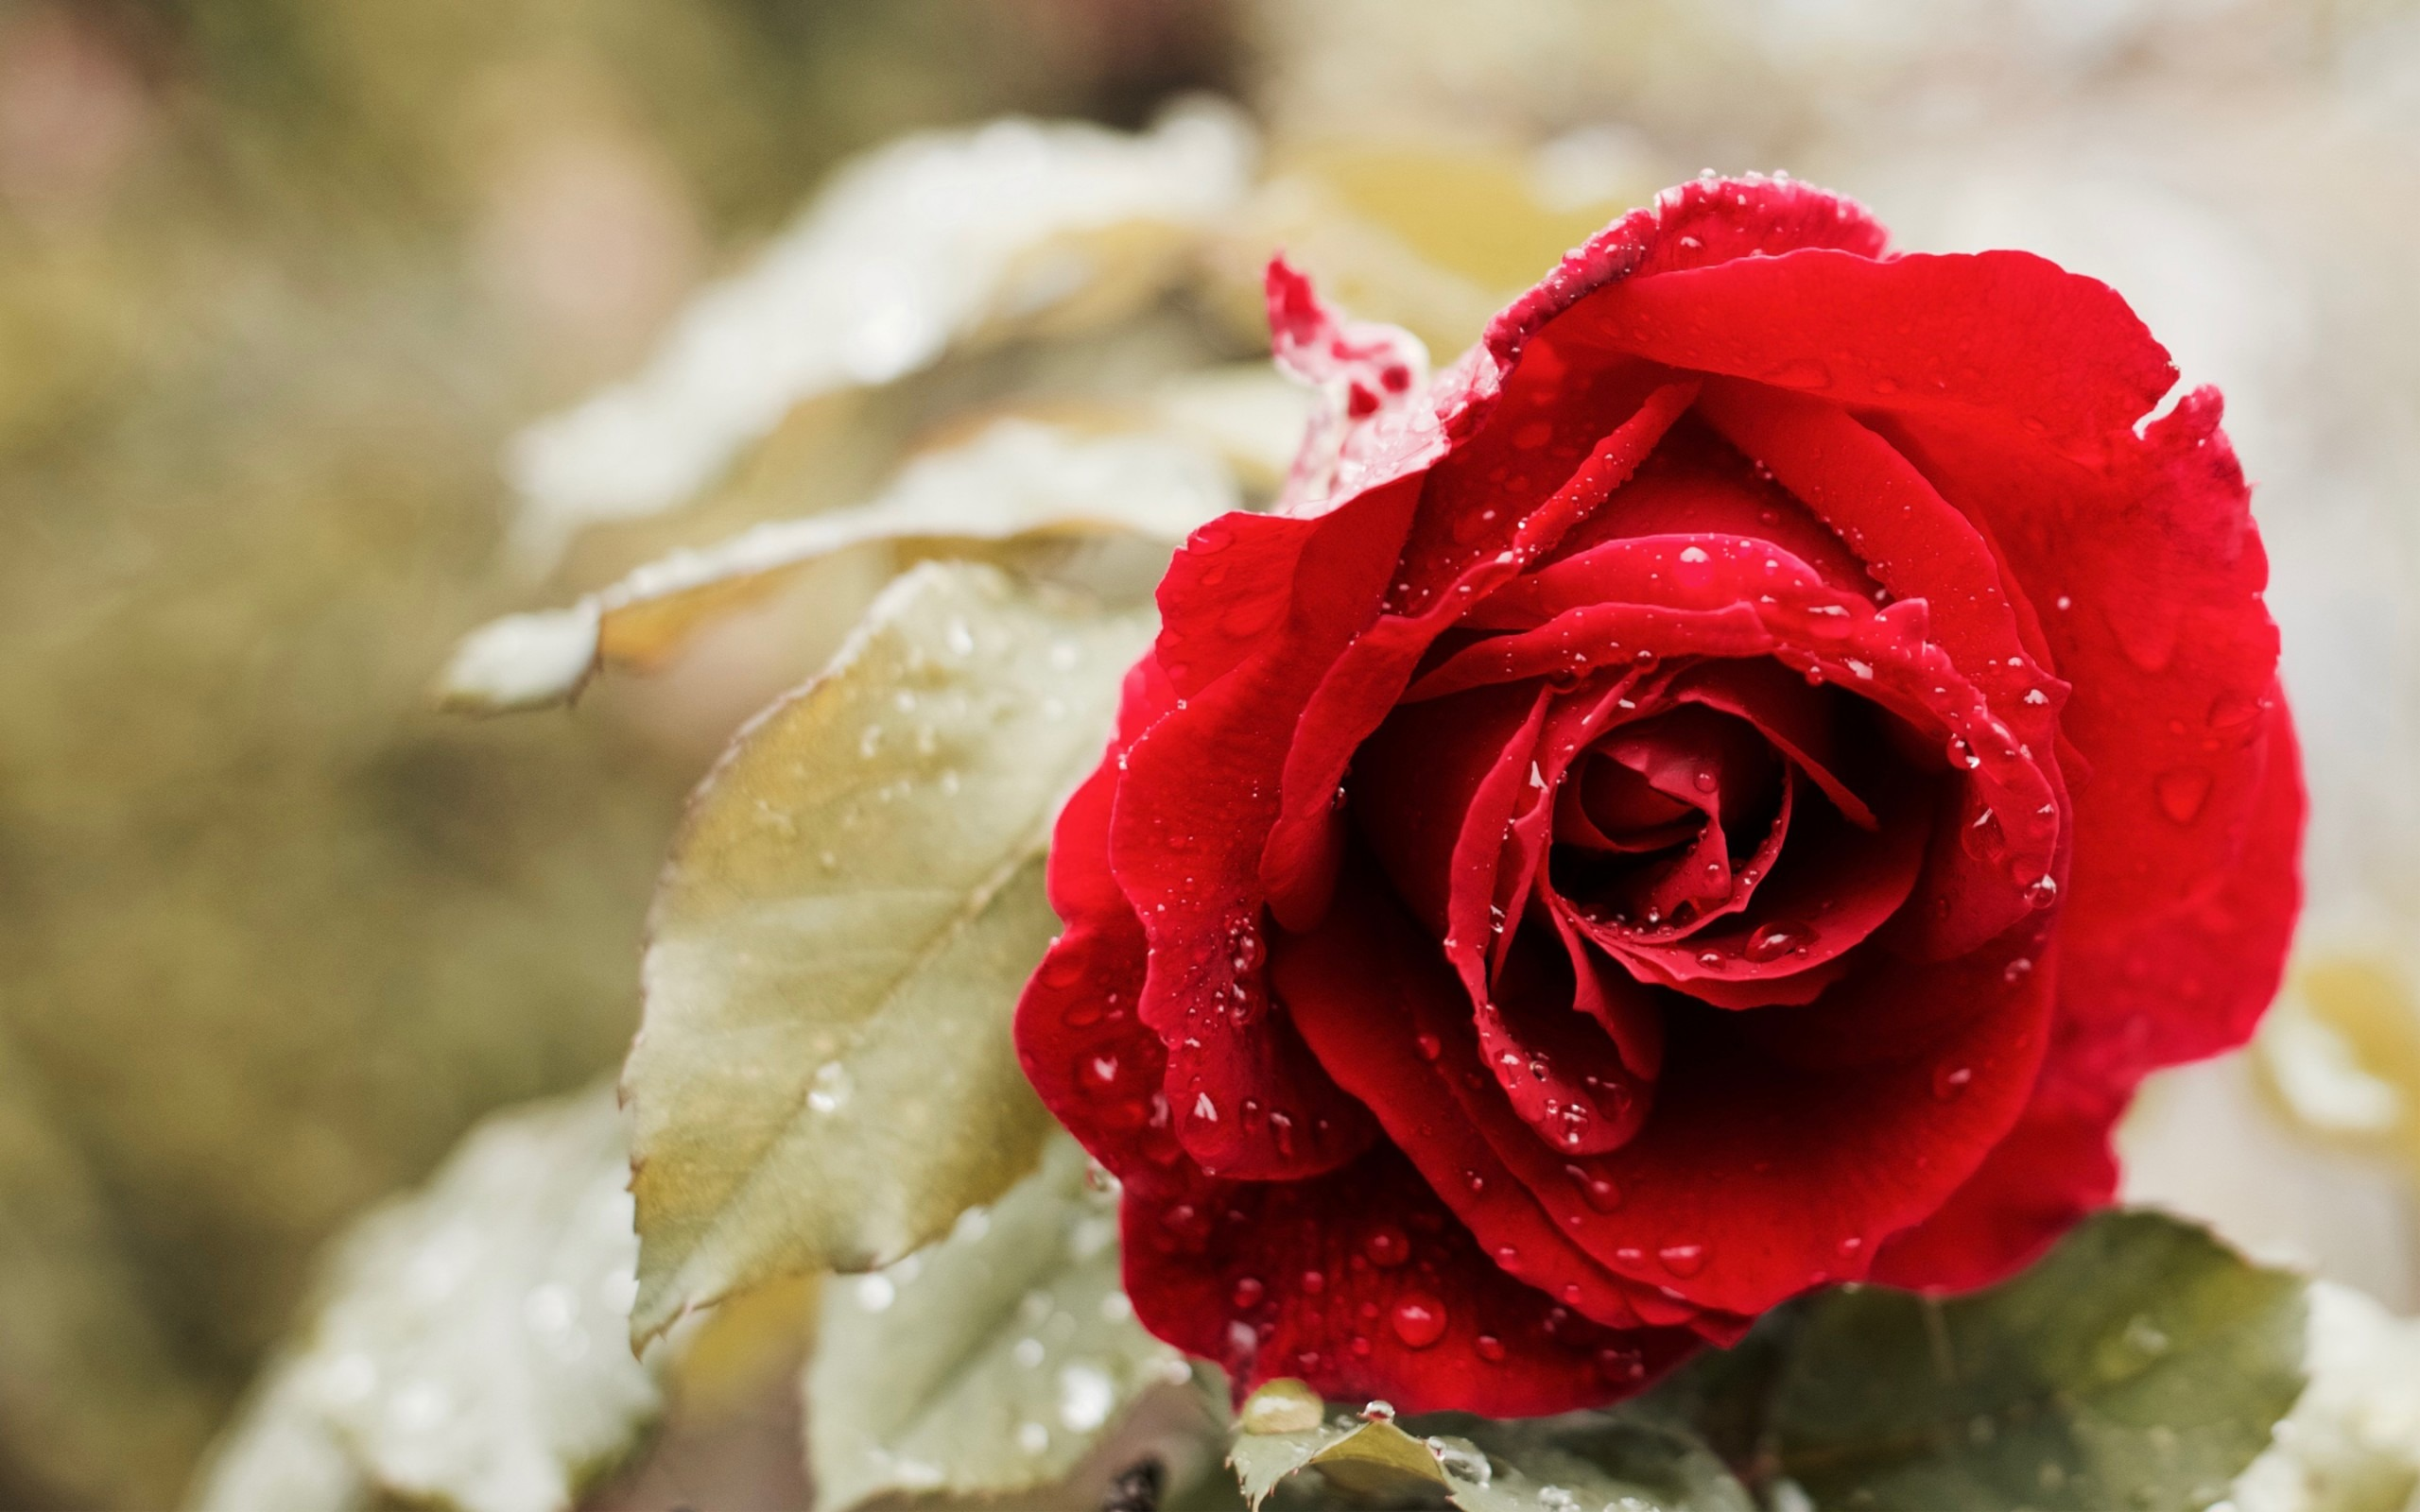
\includegraphics[width=0.5\textwidth]{imagenes/input.png}
    \caption{Imagen de entrada \texttt{input.bmp} en formato BMP de 24 bits (BGR).}
    \label{fig:input}
\end{figure}

\subsection{Salida en consola}

Tras compilar en \textbf{Release | x64} y ejecutar el programa, la consola muestra los tres mensajes del flujo:

\begin{figure}[H]
    \centering
    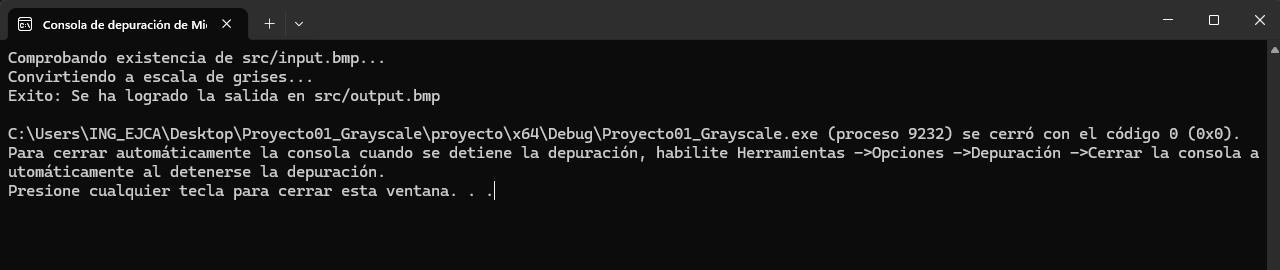
\includegraphics[width=0.8\textwidth]{imagenes/consola_ejecucion.png}
    \caption{Mensajes en consola del programa: validación, conversión y aviso de éxito.}
    \label{fig:consola}
\end{figure}

\subsection{Imagen de salida en escala de grises}

El archivo \texttt{src/output.bmp} contiene la misma imagen con los tres canales B, G y R sustituidos por el valor de gris calculado por \texttt{grayscale.asm}. Las cabeceras BMP/DIB y el padding de cada fila se conservan intactos, por lo que la imagen sigue siendo un BMP válido de 24 bits.

\begin{figure}[H]
    \centering
    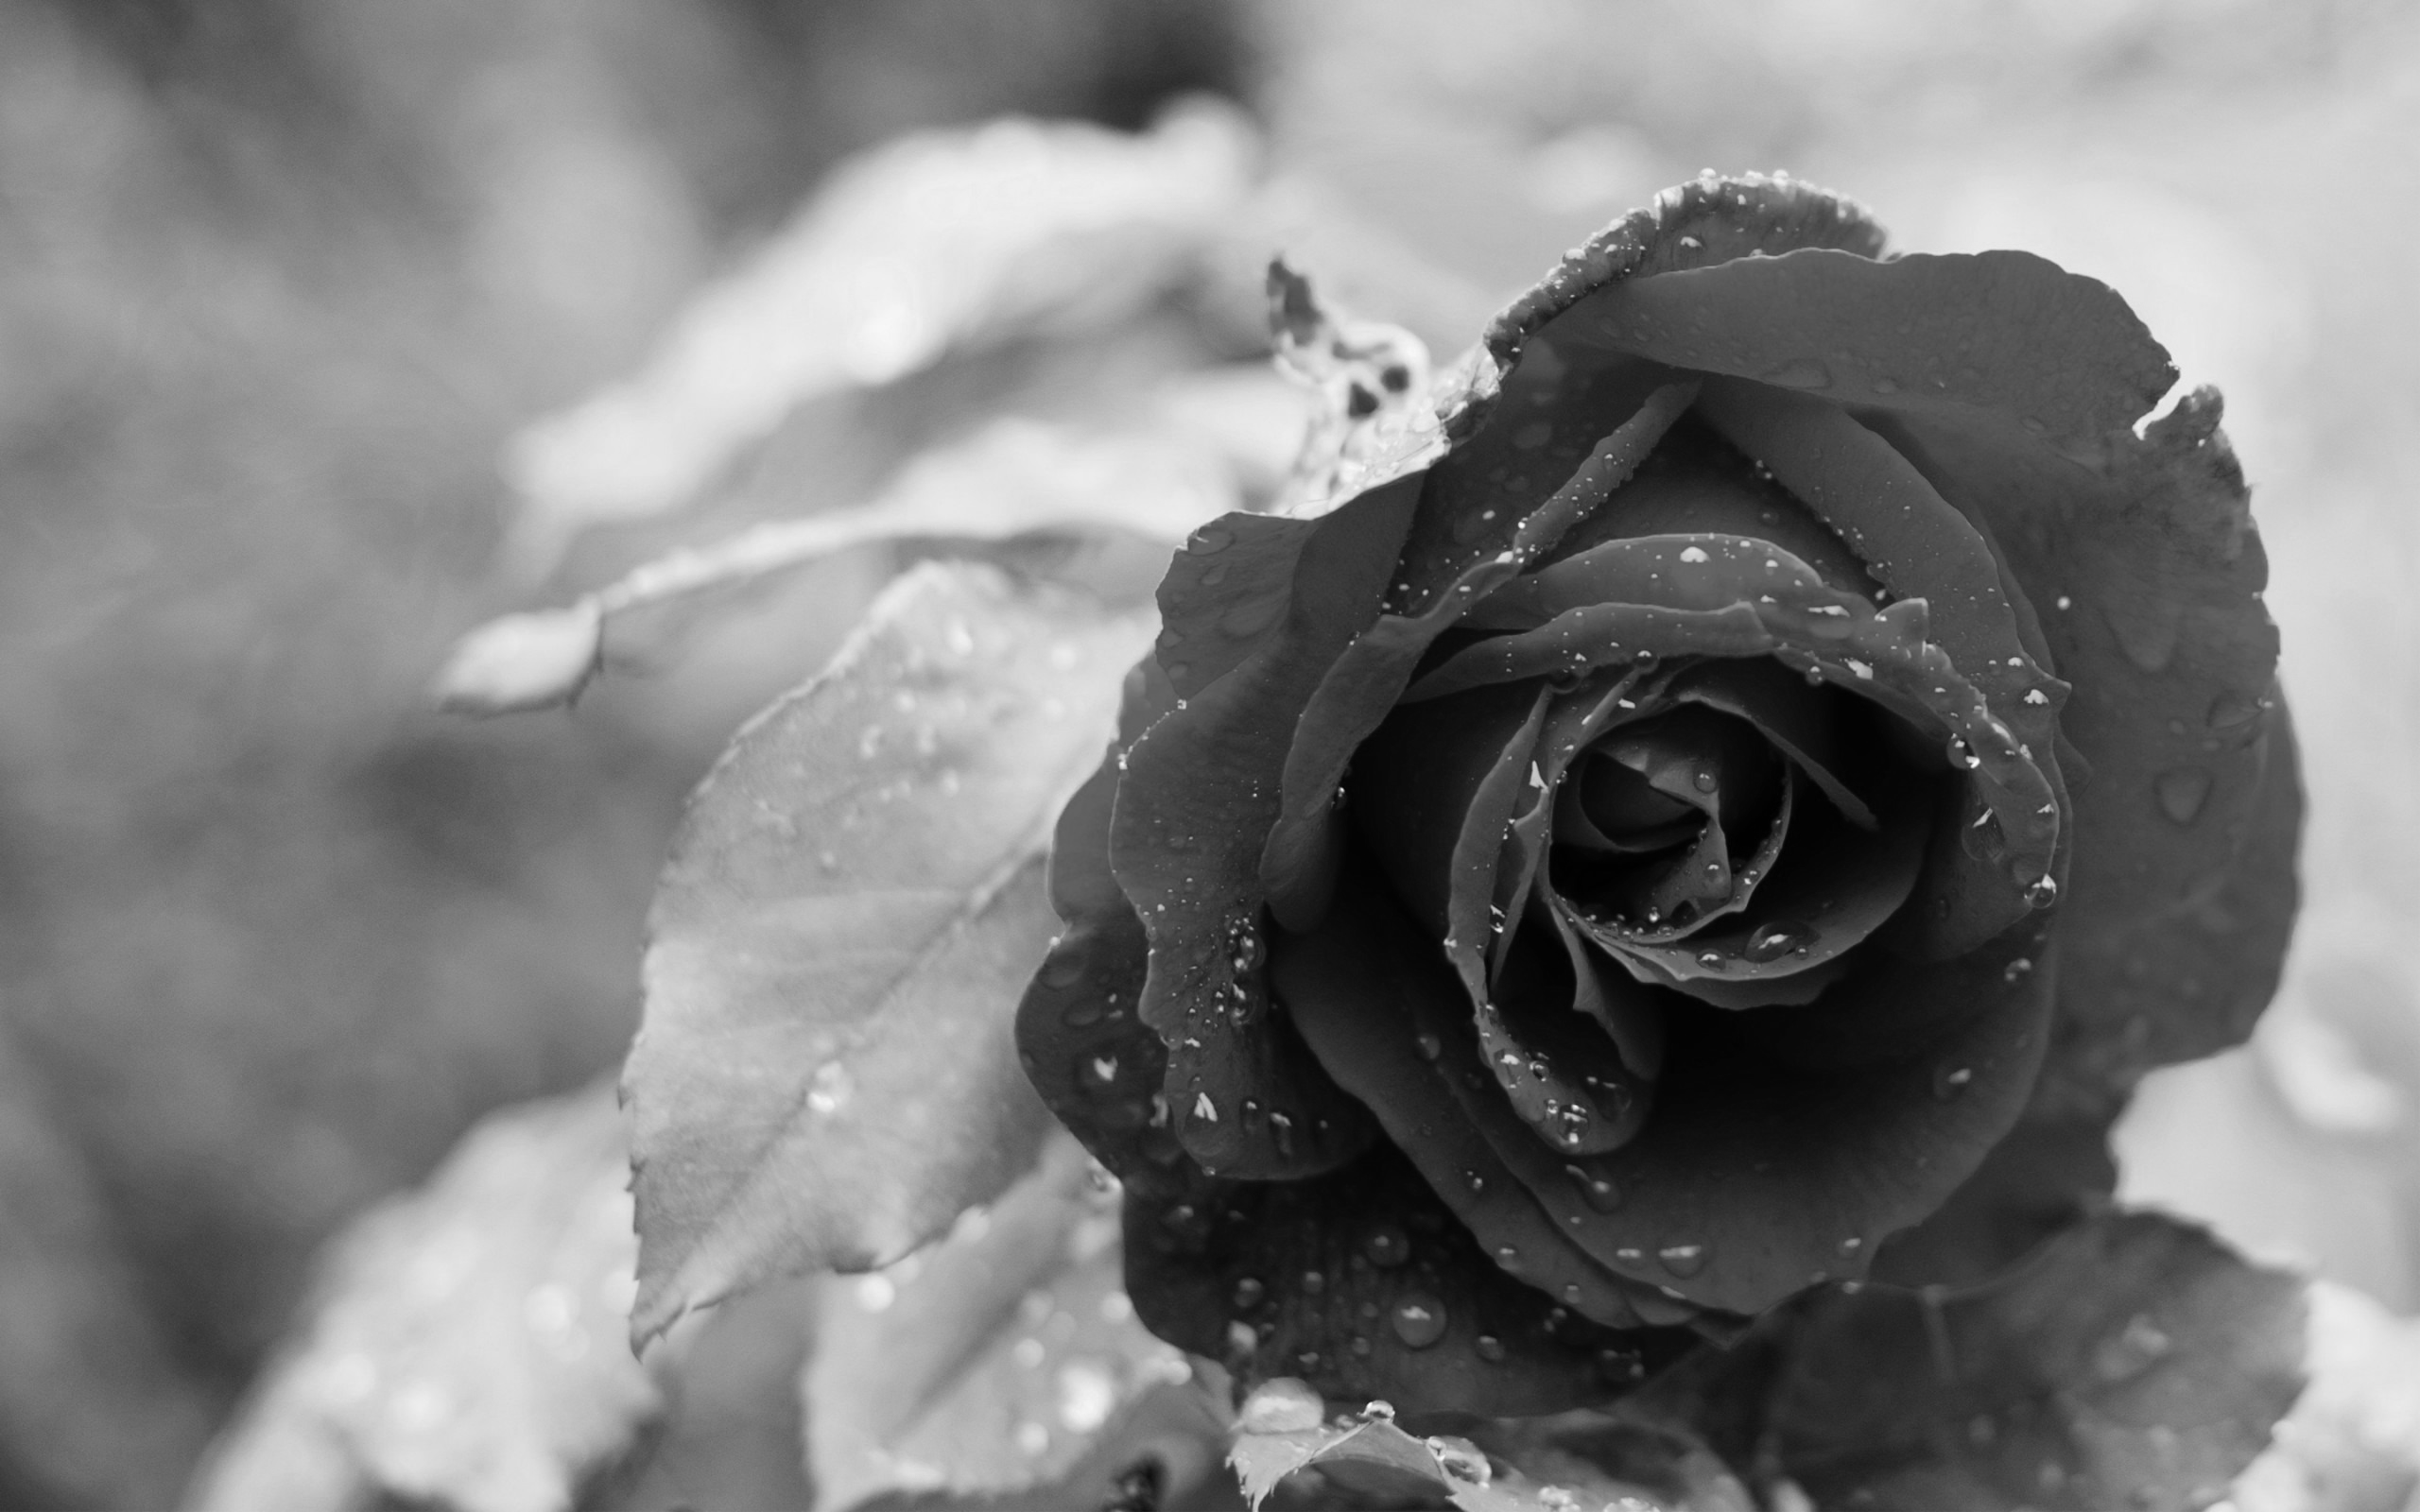
\includegraphics[width=0.5\textwidth]{imagenes/output.png}
    \caption{Imagen de salida \texttt{output.bmp} convertida a escala de grises usando los pesos ITU-R BT.601.}
    \label{fig:output}
\end{figure}

\subsection{Inspección hexadecimal de las cabeceras}

Para verificar que la estructura binaria del archivo es la esperada, se abre el BMP de entrada con un editor hexadecimal (HxD, GHex, etc.):

\begin{figure}[H]
    \centering
    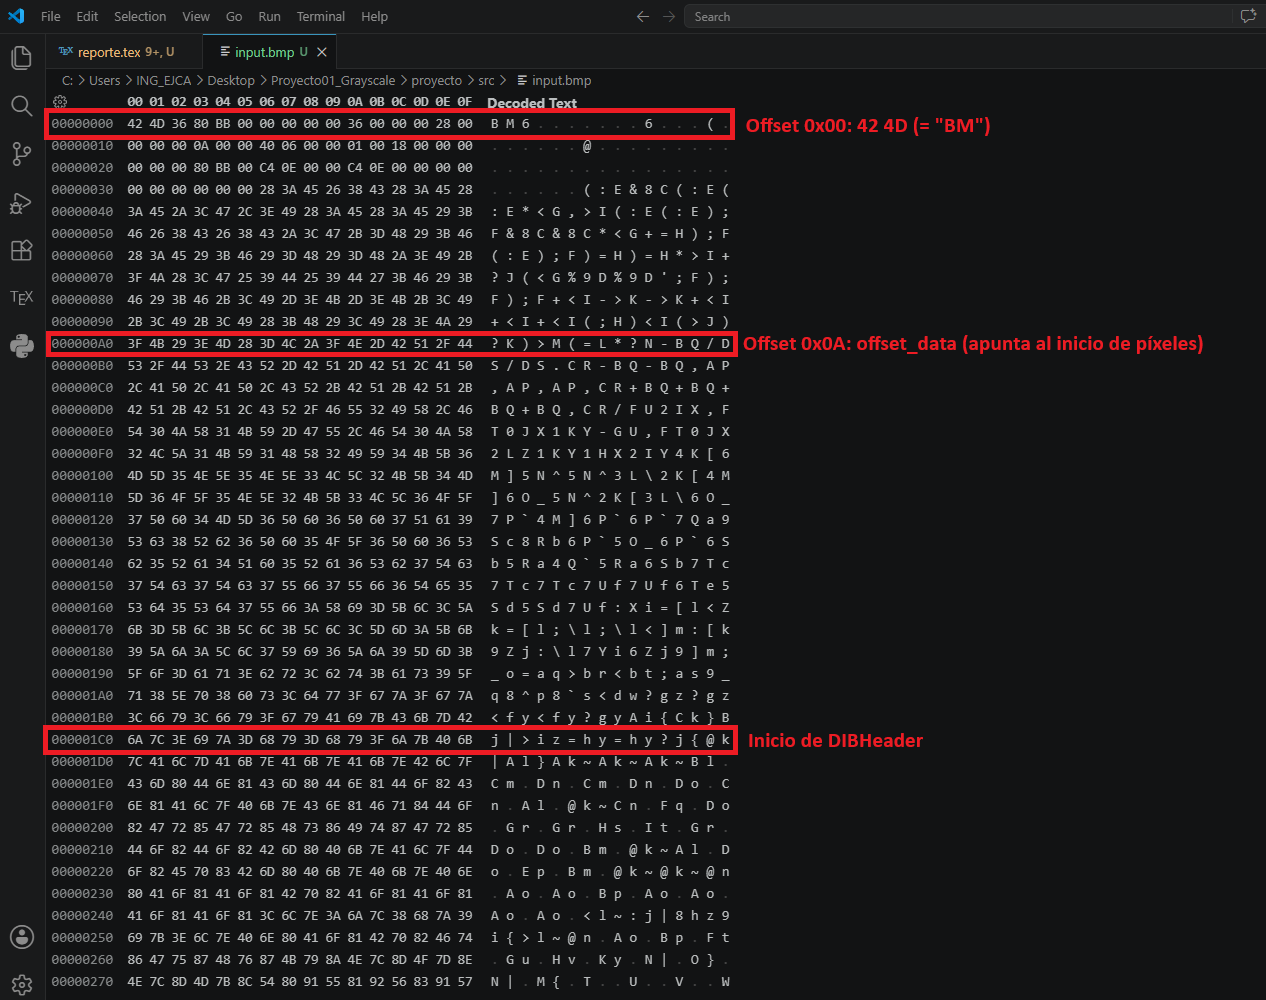
\includegraphics[width=0.8\textwidth]{imagenes/hex_header.png}
    \caption{Vista hexadecimal de \texttt{input.bmp}. Los primeros bytes \texttt{42 4D} corresponden a la firma ASCII \textit{"BM"}; en el offset \texttt{0x1C} aparece \texttt{18 00} (= 24 en little-endian), confirmando que es un BMP de 24 bits por píxel.}
    \label{fig:hex}
\end{figure}

% ============================================================
\section{Repositorio GitHub}

\url{https://github.com/7mo-ArquitecturaComputadoras/Proyecto01_Grayscale}

% ============================================================
\section{Conclusiones}

\begin{itemize}
    \item El formato \textbf{BMP de 24 bits} es un excelente vehículo didáctico porque expone explícitamente todos los detalles de bajo nivel que el procesador requiere: orden de bytes (BGR), alineación de filas a 4 bytes, almacenamiento bottom-up y la diferencia entre estructuras empaquetadas (\texttt{\#pragma pack}) y alineadas naturalmente \cite{microsoft_bmp, fileformat_bmp}.

    \item La fórmula de luminancia \textbf{ITU-R BT.601} $Y' = 0.299\,R + 0.587\,G + 0.114\,B$ no es arbitraria: refleja la sensibilidad espectral del ojo humano y produce escalas de grises perceptualmente correctas.

    \item Escalar los pesos por $2^8$ permite implementar la fórmula con \textbf{aritmética entera}, sustituyendo la división por una instrucción \texttt{SHR} de un solo ciclo. La precisión perdida es despreciable porque el error de redondeo máximo por píxel es de $\pm 1$ en una escala de 256 niveles.

    \item La elección de la convención \textbf{Microsoft x64} obliga a usar \texttt{RCX}, \texttt{RDX} y \texttt{R8} para los tres parámetros, lo que es notablemente más eficiente que el modelo \texttt{cdecl} de 32 bits porque evita lecturas/escrituras a la pila para cada llamada \cite{msft_x64_calling}.

    \item Procesar la imagen \textbf{fila por fila} en C++ y delegar a ensamblador solo el bucle interno es un compromiso pragmático: el código en C++ maneja la complejidad del formato (cabeceras, padding, archivos) mientras que el ensamblador se concentra en el trabajo verdaderamente intensivo. Este patrón es común en bibliotecas de procesamiento de imágenes profesionales.
\end{itemize}

% ============================================================
\begin{thebibliography}{99}

\bibitem{microsoft_bmp}
Microsoft Corporation, ``Bitmap Storage,'' \textit{Windows GDI Documentation}.
\url{https://learn.microsoft.com/en-us/windows/win32/gdi/bitmap-storage}

\bibitem{microsoft_bitmapinfoheader}
Microsoft Corporation, ``BITMAPINFOHEADER structure,'' \textit{Windows GDI Reference}.
\url{https://learn.microsoft.com/en-us/windows/win32/api/wingdi/ns-wingdi-bitmapinfoheader}

\bibitem{microsoft_bitmapinfo}
Microsoft Corporation, ``BITMAPINFO structure,'' \textit{Windows GDI Reference}.
\url{https://learn.microsoft.com/en-us/windows/win32/api/wingdi/ns-wingdi-bitmapinfo}

\bibitem{fileformat_bmp}
``BMP File Format Specification,'' \textit{File Format Documentation}.
\url{https://docs.fileformat.com/image/bmp/}

\bibitem{intel_manual}
Intel Corporation, \textit{Intel\textregistered{} 64 and IA-32 Architectures Software Developer's Manual, Volume 2: Instruction Set Reference}. Santa Clara, CA, 2024.
\url{https://www.intel.com/content/www/us/en/developer/articles/technical/intel-sdm.html}

\bibitem{msft_x64_calling}
Microsoft Corporation, ``x64 calling convention,'' \textit{Microsoft C++ Documentation}.
\url{https://learn.microsoft.com/en-us/cpp/build/x64-calling-convention}

\bibitem{wikipedia_data_alignment}
``Data structure alignment,'' \textit{Wikipedia, The Free Encyclopedia}.
\url{https://en.wikipedia.org/wiki/Data_structure_alignment}

\end{thebibliography}

\end{document}
